\documentclass[tikz,border=8pt]{standalone}
% Shared look for every TikZ diagram. Load with \input{../../tools/tikz-style.tex}
\usepackage[T1]{fontenc}
\usepackage{lmodern}
\renewcommand{\sfdefault}{lmr}  % diagrams use the same serif as the text
\usetikzlibrary{arrows.meta, positioning, shapes.geometric, calc, fit, backgrounds}
\definecolor{cblue}{HTML}{4C78A8}
\definecolor{corange}{HTML}{F58518}
\definecolor{cgreen}{HTML}{54A24B}
\definecolor{cred}{HTML}{E45756}
\definecolor{cpurple}{HTML}{B279A2}
\definecolor{cgrey}{HTML}{6B6B6B}
\tikzset{
  every picture/.style={font=\sffamily, line width=1.2pt},
  box/.style={draw=#1, fill=#1!12, rounded corners=4pt, align=center, inner sep=7pt, minimum height=1.1cm},
  box/.default=cgrey,
  arrow/.style={-{Stealth[length=3mm]}, draw=cgrey, line width=1.4pt},
  title/.style={font=\sffamily\bfseries\Large},
  note/.style={font=\sffamily\small, text=cgrey, align=center},
}
\AtBeginDocument{\hyphenpenalty=10000 \exhyphenpenalty=10000}

\begin{document}
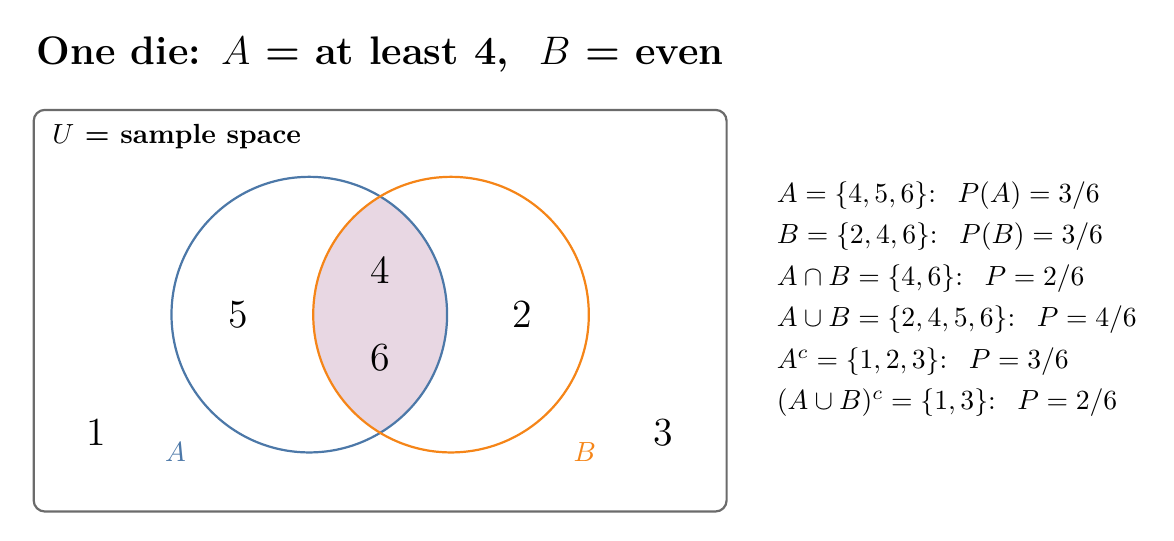
\begin{tikzpicture}[x=1cm, y=1cm]
  \node[title] at (0,3.3) {One die: $A$ = at least 4, \ $B$ = even};
  \draw[thick, rounded corners, draw=cgrey] (-4.4,-2.5) rectangle (4.4,2.6);
  \node[font=\sffamily\bfseries, anchor=north west] at (-4.3,2.55) {$U$ = sample space};
  \begin{scope}
    \clip (-0.9,0) circle (1.75);
    \fill[cpurple!30] (0.9,0) circle (1.75);
  \end{scope}
  \draw[thick, cblue] (-0.9,0) circle (1.75);
  \draw[thick, corange] (0.9,0) circle (1.75);
  \node[text=cblue, font=\sffamily\bfseries] at (-2.6,-1.75) {$A$};
  \node[text=corange, font=\sffamily\bfseries] at (2.6,-1.75) {$B$};
  \node[font=\sffamily\Large] at (-1.8,0) {5};
  \node[font=\sffamily\Large] at (0,0.55) {4};
  \node[font=\sffamily\Large] at (0,-0.55) {6};
  \node[font=\sffamily\Large] at (1.8,0) {2};
  \node[font=\sffamily\Large] at (-3.6,-1.5) {1};
  \node[font=\sffamily\Large] at (3.6,-1.5) {3};
  \node[align=left, right, font=\sffamily] at (4.9,0.2) {
    $A = \{4, 5, 6\}$: \ $P(A) = 3/6$\\[3pt]
    $B = \{2, 4, 6\}$: \ $P(B) = 3/6$\\[3pt]
    $A \cap B = \{4, 6\}$: \ $P = 2/6$\\[3pt]
    $A \cup B = \{2, 4, 5, 6\}$: \ $P = 4/6$\\[3pt]
    $A^c = \{1, 2, 3\}$: \ $P = 3/6$\\[3pt]
    $(A \cup B)^c = \{1, 3\}$: \ $P = 2/6$};
\end{tikzpicture}
\end{document}
